\documentclass[10pt,journal,compsoc]{IEEEtran}

\usepackage{verbatim}
\usepackage{url}
\usepackage{graphicx}

\usepackage{xspace}
\newcommand{\FC}       {Freechains\xspace}
\newcommand{\reps}     {\emph{reps}\xspace}
\newcommand{\onerep}   {\emph{1~rep}\xspace}
\newcommand{\nreps}[1] {\emph{#1~reps\xspace}}
\newcommand{\code}[1]  {\texttt{\footnotesize{#1}}}
\newcommand{\Xon} {$1{\rightarrow}N$\xspace}
\newcommand{\Xno} {$1{\leftarrow}N$\xspace}
\newcommand{\Xnn} {$N{\leftrightarrow}N$\xspace}
\newcommand{\Xoo} {$1{\leftrightarrow}1$\xspace}
\newcommand{\Xo}  {$1{\hookleftarrow}$\xspace}

\renewcommand{\theenumi}{\alph{enumi}}

\hyphenation{off-line}

\begin{document}

\title{
    Symmetric Peer-to-Peer Applications
}

\author{
    Francisco Sant'Anna~\IEEEmembership{Department of Computer Science, Rio de Janeiro State University}
}

\IEEEtitleabstractindextext{%
\begin{abstract}
In multi-node collaborative applications, users can interact asynchronously
and share the exact same experience remotely.
%
In this work, we propose a middleware for \emph{symmetric peer-to-peer
applications} in which decentralized instances can broadcast asynchronous
events and yet conform to identical behavior.
%
Nodes are allowed to join and leave the network at any time.
Application developers must adhere to a restricted API, which is
deterministic, stateless, and only supports pre-allocated memory.
%
The middleware is responsible for synchronizing the events in a global shared
timeline across the network.
Based on memory snapshots and deterministic simulation, a ``time machine''
rolls back and resynchronizes the state of conflicting nodes.
%
TODO: application, results
\end{abstract}

\begin{IEEEkeywords}
collaboration, determinism, peer-to-peer, time machine
\end{IEEEkeywords}}

\maketitle

% TOTAL: 12 pages

\section{Introduction}
\label{sec.introduction}

\IEEEPARstart{C}{ollaborative} networked applications allow multiple users to
interact remotely and yet share the same experience in real time.
Examples of such \emph{symmetric distributed applications}~\cite{gals}
are shared documents, watch parties, and multi-player games.
%
In order to reproduce the exact behavior in multiple devices, the application
must be able to synchronize its time and execution across the network.
In addition, since users can interact asynchronously with the application,
event occurrences must somehow be synchronized back across devices.

A common approach towards symmetric applications is to introduce a middleware
to orchestrate events and time in the network~\cite{gals,croquet}.
Applications developers rely on middleware primitives to trigger events, which
are intercepted and synchronized in a global shared timeline across the
network.
Developers must also restrict themselves to deterministic and stateless calls
only, such that execution can be equally reproduced in all nodes according to
the shared timeline.
However, current solutions depend on a central server to interconnect network
nodes and determine the shared timeline.

In this work, we propose \emph{symmetric peer-to-peer applications}, which
do not rely on central servers for coordination.
Nodes in the application form a dynamic peer-to-peer network and communicate
only with their neighbours directly.
Events are flooded in the network and are triggered locally with a small
delay to cope with latency.
Our main contribution is a time machine that can rollback nodes to a previous
state to apply events received out of order or too late.

TODO: application, results

In Section~\ref{sec.related}, we revisit existing solutions for symmetric
distributed applications.
In Section~\ref{sec.tml}, we detail our proposed middleware.
In Section~\ref{sec.app}, ...
In Section~\ref{sec.eval}, ...
In Section~\ref{sec.conclusion}, ...

- assumptions
    - correct (non-malicious) nodes

- local first
- p2p
- less restrictive (compared to CRDTs)
- semantic events
    - limitation b/c of rollbacks
    - features b/c of network traffic

\section{Related Work}
\label{sec.related}

% docs.google.com/spreadsheets/d/1CpMmEgabJq2XQeTDW_BNCV4JWrcMlELuaEjDtw7kwg0/
\begin{figure}[t]
  \centering
  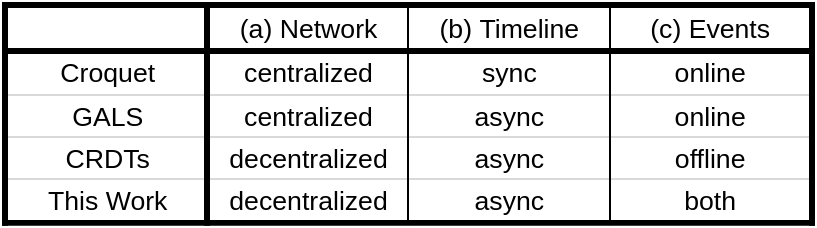
\includegraphics[width=\linewidth]{table}
  \caption{
    \label{fig.table}
  }
\end{figure}

\begin{figure*}[t]
  \centering
  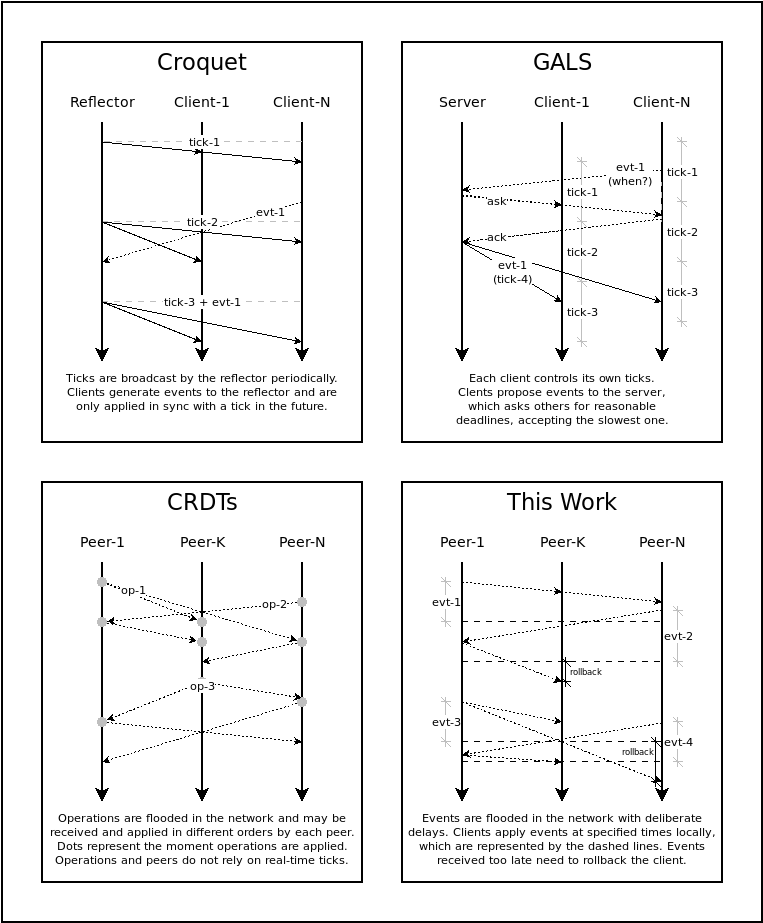
\includegraphics[width=\linewidth]{algos}
  \caption{
    \label{fig.algos}
  }
\end{figure*}

In this section, we revisit existing solutions for symmetric distributed
applications.
We focus on (i) how the network is organized, (ii) how global time is
determined, and (iii) how events are propagated.
Figure~\ref{fig.table} compares selected works regarding these aspects.

Croquet%
\footnote{Croquet.io: https://croquet.io/}~\cite{croquet} guarantees
bit-identical real-time behavior for every user in a collaborative
distributed environment.
%
As detailed in Figure~\ref{fig.algos}, a centralized \emph{reflector} issues
periodic ticks, such that all nodes in the network advance together according
to a synchronized global shared clock.
If an user generates an event, it is delayed and sent back to the reflector,
which broadcasts the event in the next tick, which all nodes apply in sync
(including the originating node).
%
Croquet takes periodic snapshots of the whole application state in order to
support late joins to a running session.
The new node just needs to restore the latest snapshot and simulate the
remaining events to reach the current running state.
%
As indicated in Figure~\ref{fig.table}, Croquet relies on a centralized
network, in which nodes advance in sync, and in which event outcomes depend
on the originating node to be online.

GALS~\cite{gals} shares the same goals with Croquet, but with some tradeoffs,
mostly favoring clients with slow connections.
As detailed in Figure~\ref{fig.algos}, instead of advancing ticks in sync with
the server, clients have their own local clocks.
Also, event generation is delayed dynamically according to the slowest client.
%
On the one hand, ticks do not generate any traffic and clients have smooth
frame transitions, even those with poor connections.
On the other hand, event generation requires two round trips to the server and
clients may experience occasional freezes.
The syncing protocol also requires bookkeeping to deal with clock drifts and
client disconnections.
%
As indicated in Figure~\ref{fig.table}, GALS relies on a centralized
network, in which nodes advance independently, and in which event outcomes
depend on the originating node to be online.

In both solutions, the application advances in real time, with a total order
among events, which is determined by a centralized server that must be
permanently online.
All clients compute the events in sequence, respecting their timestamps, and
using only deterministic and stateless calls.
This way, it is guaranteed that all clients reach the same state, going
through bit-identical steps.

An antagonistic approach to deterministic reactions to events is to model the
application data structures with conflict-free replicated data types
(CRDTs)~\cite{crdts}.
CRDTs are designed in such a way that all operations are commutative, so that
the order in which they are applied does not affect the final outcome.
%
As detailed in Figure~\ref{fig.algos}, peers can communicate operations
directly to each other with no central authority.
Also, since operations need not to be ordered, they can be applied at the
very first moment they are generated or received, even if the peers are
offline.
%
Since operations must be commutative, it is not possible to timestamp them
in a global shared clock.
Hence, there is no notion of a timeline with peers going through bit-identical
steps, but they do eventually reach the same state.
%
On the one hand, the main advantage of CRDTs is they support the concept of
local-first software~\cite{local}, since they work offline.
On the other hand, they provide very restrictive APIs (the CRDTs themselves),
and do not support real-time consensus among peers.
%
As indicated in Figure~\ref{fig.table}, CRDTs work on decentralized networks,
in which nodes advance independently, and in which operations can be applied
immediately, even while offline.
%
Automerge along with its accompanying Hypermerge peer-to-peer infrastructure
is an example of an implementation of this approach~\cite{p2p.automerge,p2p.pushpin}.

In this work, as indicated in Figure~\ref{fig.table}, our goal is to support
peer-to-peer real-time symmetric execution, while still tolerating offline and
out-of-order event generation.
%
As detailed in Figure~\ref{fig.algos}, peers have independent timelines and
can communicate events directly to each other.
Events are delayed to be able to reach other peers in time.
In the case a deadline is missed, the peer rolls back in time and then fast
forwards execution until it reaches real time again.
%
Like Croquet and GALS, peers compute events in sequence using only
deterministic and stateless calls.

Fusion%
\footnote{Fusion: \url{https://doc.photonengine.com/en-us/fusion}}
is a state synchronization networking library for the Unity game engine.
It provides networked tick-based simulation in two modes: client-server
(\emph{hosted mode}) or peer-to-peer (\emph{shared mode}).
The hosted mode is based on continuous memory snapshots, which allows for
full rollbacks when clients diverge.
However, the shared mode is less powerful and only supports eventual
consistency among clients.
We presume that continuous memory snapshots would be too expensive without a
central server.

Regarding single-user time machines, the video game Braid%
\footnote{\url{Braid: http://braid-game.com/}}
is designed on the assumption that players have unrestricted power to go back
in time.
Like Fusion, it's implementation is based on continuous memory snapshots, and
not deterministic simulation as we propose in this work.

- time machine
    - paper que eu achei ha um tempo
    - braid

\section{The API \& Middleware}
\label{sec.tml}

\section{Application}
\label{sec.app}

\section{Evaluation}
\label{sec.eval}

\section{Conclusion}
\label{sec.conclusion}

\bibliographystyle{IEEEtran}
\bibliography{tpd-22}

\begin{comment}
\begin{IEEEbiography}[{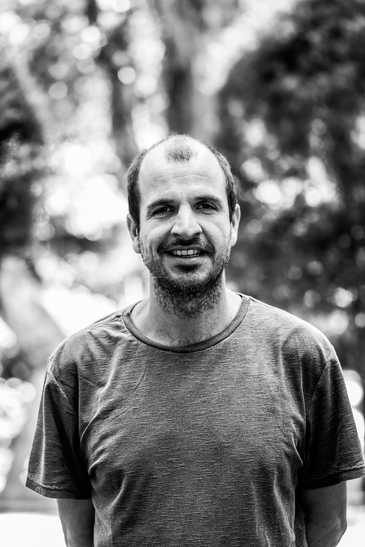
\includegraphics[width=1in,height=1.25in,clip,keepaspectratio]{chico}}]{Francisco Sant'Anna}
received his PhD degree in Computer Science from PUC-Rio, Brazil in
2013.
In 2016, he joined the Faculty of Computer Science at the Rio de Janeiro State
University, Brazil.
His research interests include Programming Languages and Concurrent \&
Distributed Systems.
\end{IEEEbiography}
\end{comment}

\end{document}
